\part{Teoretická část}

\chapter{Historie \gls{xr}}

\section{Počátky \gls{xr}}

První pokusy o rozšířenou realitu pochází už z 50. let 20. století, kdy Morton Hellig, americký kinematograf, přivádí na svět své zařízení zvané Sensorama. Nejednalo se ovšem o headset, které si vybavíme dnes -- Sensorama bylo statické zařízení, vzhledově připomínající spíše arkádový automat. Hellig toto zařízení nazýval "zážitkovým divadlem", které bylo schopno zobrazit 3D obraz, pouštět stereo zvuk a vytvářet vítr. Tím se od dnešní XR technologie zásadně liší; nepřijímá vstup uživatele. Sensorama se ovšem nedočkala úspěchu a známe ji jen jako historicky první pokusy o virtuální realitu.

\begin{figure}[H]
    \centering
    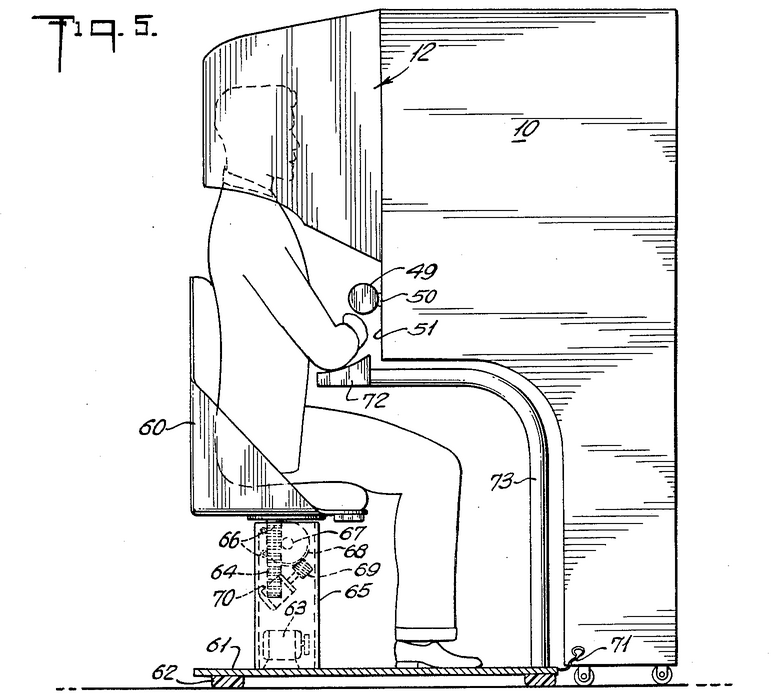
\includegraphics[height=250pt]{sensorama.png}
    \caption{Sensorama}
    \label{sensorama}
\end{figure}

Ivan Sutherland, americký vědec, který je často označován jako průkopník v oblasti počítačové grafiky. Společně se svými studenty vynalezl vůbec první zařízení pro virtuální realitu -- zvané Damoklův meč. Vzhledem jeho primitivnosti zobrazovalo pouze čtvercové místnosti tvořené z čar, které software následně transofrmoval do správné perspektivy. Pohyby sledovalo pomocí mechanické paže připevněné ke stropu, ke které byl headset připevněný.

\section{\gls{xr} dnes}

lorem ipsum

\chapter{Hardware}
lorem ipsum

něco o trackování, výrobcích, atd. zmínit trackovací systém bez věží od Meta/FB

rozlišit 6dof vs 3dof

\chapter{Software}
lorem ipsum

zmínit OpenXR, WebXR jakožto API co pohánějí XR

rozlišit PCVR na windows a mobilní VR na bázi androidu